\documentclass{beamer}
\mode<presentation>
\usepackage{amsmath}
\usepackage{amssymb}
%\usepackage{advdate}
\usepackage{adjustbox}
\usepackage{subcaption}
%\usepackage{enumitem}
\usepackage{multicol}
\usepackage{mathtools}
\usepackage{listings}
\usepackage{url}
\usepackage{tikz}
\usepackage{enumerate}
\usetikzlibrary{matrix}
\def\UrlBreaks{\do\/\do-}
\usetheme{metropolis}
%\usecolortheme{lily}
\setbeamertemplate{footline}
{
  \leavevmode%
  \hbox{%
  \begin{beamercolorbox}[wd=\paperwidth,ht=2.25ex,dp=1ex,right]{author in head/foot}%
    \insertframenumber{} / \inserttotalframenumber\hspace*{2ex} 
  \end{beamercolorbox}}%
  \vskip0pt%
}
\setbeamertemplate{navigation symbols}{}

\providecommand{\nCr}[2]{\,^{#1}C_{#2}} % nCr
\providecommand{\nPr}[2]{\,^{#1}P_{#2}} % nPr
\providecommand{\mbf}{\mathbf}
\providecommand{\pr}[1]{\ensuremath{\Pr\left(#1\right)}}
\providecommand{\qfunc}[1]{\ensuremath{Q\left(#1\right)}}
\providecommand{\sbrak}[1]{\ensuremath{{}\left[#1\right]}}
\providecommand{\lsbrak}[1]{\ensuremath{{}\left[#1\right.}}
\providecommand{\rsbrak}[1]{\ensuremath{{}\left.#1\right]}}
\providecommand{\brak}[1]{\ensuremath{\left(#1\right)}}
\providecommand{\lbrak}[1]{\ensuremath{\left(#1\right.}}
\providecommand{\rbrak}[1]{\ensuremath{\left.#1\right)}}
\providecommand{\cbrak}[1]{\ensuremath{\left\{#1\right\}}}
\providecommand{\lcbrak}[1]{\ensuremath{\left\{#1\right.}}
\providecommand{\rcbrak}[1]{\ensuremath{\left.#1\right\}}}
\theoremstyle{remark}
\newtheorem{rem}{Remark}
\newcommand{\sgn}{\mathop{\mathrm{sgn}}}
\providecommand{\abs}[1]{\left\vert#1\right\vert}
\providecommand{\res}[1]{\Res\displaylimits_{#1}} 
\providecommand{\norm}[1]{\lVert#1\rVert}
\providecommand{\mtx}[1]{\mathbf{#1}}
\providecommand{\mean}[1]{E\left[ #1 \right]}
\providecommand{\fourier}{\overset{\mathcal{F}}{ \rightleftharpoons}}
%\providecommand{\hilbert}{\overset{\mathcal{H}}{ \rightleftharpoons}}
\providecommand{\system}{\overset{\mathcal{H}}{ \longleftrightarrow}}
	%\newcommand{\solution}[2]{\textbf{Solution:}{#1}}
%\newcommand{\solution}{\noindent \textbf{Solution: }}
\providecommand{\dec}[2]{\ensuremath{\overset{#1}{\underset{#2}{\gtrless}}}}
\newcommand{\myvec}[1]{\ensuremath{\begin{pmatrix}#1\end{pmatrix}}}
\newcommand*{\permcomb}[4][0mu]{{{}^{#3}\mkern#1#2_{#4}}}
\newcommand*{\perm}[1][-3mu]{\permcomb[#1]{P}}
\newcommand*{\comb}[1][-1mu]{\permcomb[#1]{C}}
\let\vec\mathbf

\lstset{
%language=C,
frame=single, 
breaklines=true,
columns=fullflexible
}

\numberwithin{equation}{section}

\title{Computational probability \brak{\text{11.16.3.8.9}}}
\author{Agamjot Singh,\\EE24BTECH11002,\\IIT Hyderabad.}

\date{\today} 
\begin{document}

\begin{frame}
\titlepage
\end{frame}

\section*{Outline}
\begin{frame}
\frametitle{Table of Contents}
\tableofcontents
\end{frame}

\section{Problem}

\begin{frame}
\frametitle{Problem Statement}
Three coins are tossed at once. Find the probability of getting atmost two tails.
\end{frame}

\section{Solution}

% --- 
\subsection{Defining the sample event space, and random variables}
\begin{frame}
\frametitle{Defining the sample event space, and random variables}
Sample space $\brak{\Omega}$ is given by,
\begin{align}
    \Omega = \cbrak{HHH, HHT, HTH, HTT, THH, THT, TTH, TTT}
\end{align}
Event space $\brak{\mathcal{F}}$ is given by,
\begin{align}
    \mathcal{F} = 2^{\Omega}
\end{align}
Let $X$ be the random variable,
\begin{align}
    X = \text{number of tails in the sequence}
\end{align}
\end{frame}

% ---
\begin{frame}
We express this random variable as a sum of $3$ bernoulli random variables.
\begin{align}
    X = X_1 + X_2 + X_3
\end{align}
where,
\begin{align}
    X_{i} = \begin{cases}
        0 & \quad i^{\text{th}} \text{ toss is a Heads}\\
        1 & \quad i^{\text{th}} \text{ toss is a Tails}
    \end{cases}
\end{align}
$X$ models a binomial distribution.
\end{frame}

% ---
\subsection{Z-transform to calculate PMF}
\begin{frame}
\frametitle{Z-transform to calculate PMF}
For converting to $z$-domain, we use the property,
\begin{align}
    M_{X}\brak{z} = M_{X_1}\brak{z} M_{X_2}\brak{z} M_{X_3}\brak{z}
\end{align}
Extending this system to $m$ tosses, we get, 
\begin{align}
    M_{X}\brak{z} = \prod_{k = 1}^{m} M_{X_{k}}\brak{z}
\end{align}
Let probablity mass function function for the bernoulli random variable $X_{i}$ be given by,
\begin{align}
    p_{X_{i}}\brak{n} = \begin{cases}
        p & \quad n = 0\\
        1 - p & \quad n = 1\\
        0 & \quad n = \mathbb{Z} - \cbrak{0, 1}
    \end{cases}
\end{align}
where $p$ is the probablity of getting heads.

\end{frame}

% ---
\begin{frame}
\begin{align}
    M_{X_1}\brak{z} &= \sum_{k = -\infty}^{\infty} p_{X_{1}}\brak{n} z^{-k} = p + \brak{1 - p} z^{-1}\\
    M_{X_2}\brak{z} &= \sum_{k = -\infty}^{\infty} p_{X_{2}}\brak{n} z^{-k} = p + \brak{1 - p} z^{-1}\\
                    &\vdots\\
    M_{X_m}\brak{z} &= \sum_{k = -\infty}^{\infty} p_{X_{m}}\brak{n} z^{-k} = p + \brak{1 - p} z^{-1}\\
    \implies M_{X}\brak{z} &= \brak{p + \brak{1 - p} z^{-1}}^{m}\\
    M_{X}\brak{z} &= \sum_{k = -\infty}^{\infty} \brak{\comb{m}{k} p^{m - k} \brak{1 - p}^{k}} z^{-k}\\
\end{align}
\end{frame}

% ---
\begin{frame}
Taking $z$-inverse on both sides, we get,
\begin{align}
    p_{X}\brak{n} = \comb{m}{n} p^{m - n} \brak{1 - p}^{n}
\end{align}
Taking $m = 3$ and $p = \frac{1}{2}$,
\begin{align}
    p_{X}\brak{n} = \comb{3}{n} \brak{\frac{1}{2}}^{3}
\end{align}
Using this probability mass function, the cummulative distribution function C.D.F $\brak{F_{X}\brak{n}}$ is given by,
\begin{align}
    F_{X}\brak{n} &= \sum_{k = -\infty}^{n}  \comb{3}{k} \brak{\frac{1}{2}}^{3}\\
\end{align}
\end{frame}

% ---
\begin{frame}
    \begin{align}
        F_{X}\brak{n} &= \begin{cases}
            0 & n < 0\\
            \comb{3}{0}\brak{\frac{1}{2}}^3 = \frac{1}{8} & 0 \leq n < 1\\
            \comb{3}{0}\brak{\frac{1}{2}}^3 + \comb{3}{1}\brak{\frac{1}{2}}^3 = \frac{1}{2} & 1 \leq n < 2\\
            \comb{3}{0}\brak{\frac{1}{2}}^3 + \comb{3}{1}\brak{\frac{1}{2}}^3 + \comb{3}{2}\brak{\frac{1}{2}}^3 = \frac{7}{8} & 2 \leq n < 3\\
            \comb{3}{0}\brak{\frac{1}{2}}^3 + \comb{3}{1}\brak{\frac{1}{2}}^3 + \comb{3}{2}\brak{\frac{1}{2}}^3 + \comb{3}{3}\brak{\frac{1}{2}}^3 = 1 & 3 \leq n
        \end{cases}
    \end{align}
Let $A$ be an event defined as,
\begin{align}
    A&\colon\text{Getting atmost two tails}\\
    \pr{A} &= \pr{X<=2} = F_{X}\brak{2}\\
    \pr{A} &= \frac{7}{8} = 0.875
\end{align}

\end{frame}

% ---
\subsection{Simulation}
\begin{frame}
\frametitle{Simulation}
Running a simulation requires generating random numbers with uniform probability. This is done using OpenSSL's random byte generator.
\begin{enumerate}
    \item $1$ byte of randomly generated uniform data is generated using OpenSSL rand.h.
    \item This random number is scaled down from $\cbrak{0, 1, 2, \dots 255}$ to $\sbrak{0, 1}$ by dividing by 255.
    \item For generating the bernoulli random variable, if this normalized number is less than $p$ then 0 is returned, else 1 is returned.
\end{enumerate}
As number of trials increase, the relative frequency converges to the actual probability of the event.
\end{frame}

% ---
\subsection{Plot}
\begin{frame}
\frametitle{Plot}
\begin{figure}[h!]
  \centering
  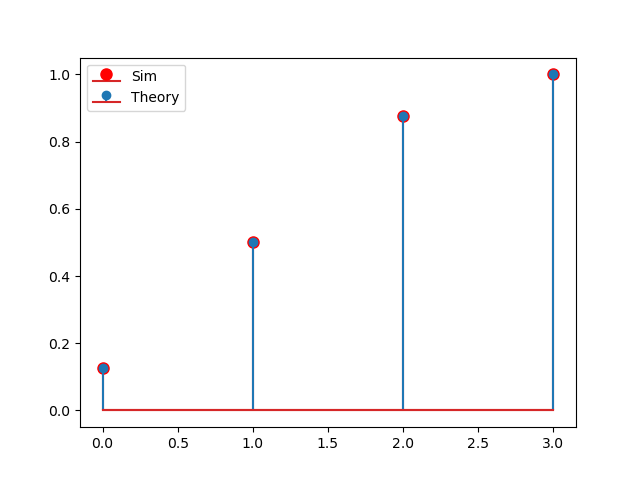
\includegraphics[width=0.7\columnwidth]{figs/cdf.png}
  \caption{CDF Plot}
  \label{label}
\end{figure}
\end{frame}

% ---
\begin{frame}
\begin{figure}[h!]
  \centering
  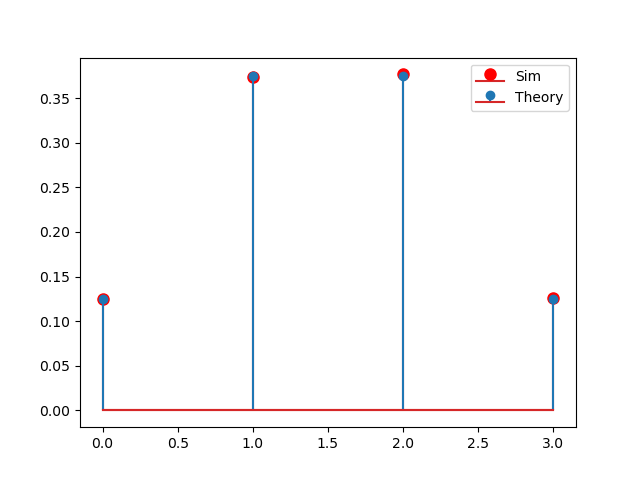
\includegraphics[width=0.7\columnwidth]{figs/pmf.png}
  \caption{PMF plot for $m$ = 3}
  \label{label}
\end{figure}
\end{frame}

% ---
\begin{frame}
\begin{figure}[h!]
    {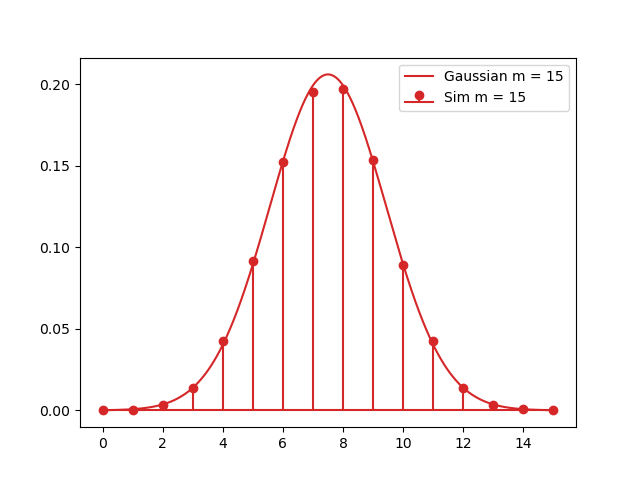
\includegraphics[width=0.4\columnwidth]{./figs/gauss_0.png}}
    \hspace{\fill}
    {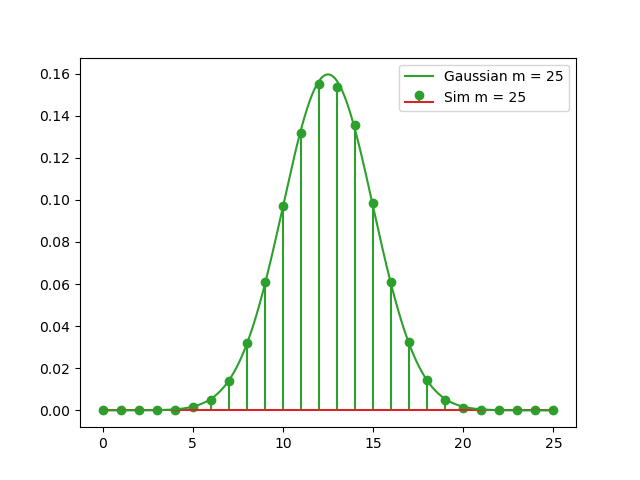
\includegraphics[width=0.4\columnwidth]{./figs/gauss_1.png}}
\end{figure}
\begin{figure}[h!]
    {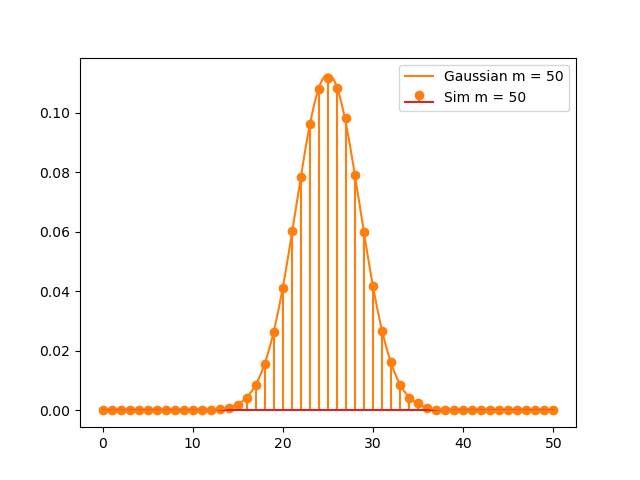
\includegraphics[width=0.4\columnwidth]{./figs/gauss_2.png}}
    \hspace{\fill}
    {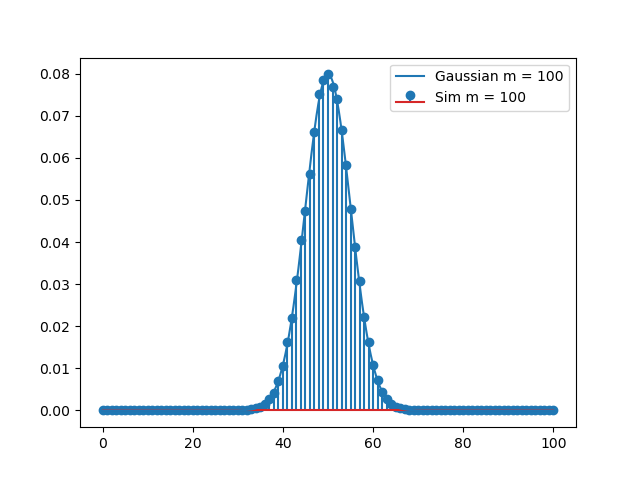
\includegraphics[width=0.4\columnwidth]{./figs/gauss_3.png}}
    \caption{Simulated PMF as well as Gaussian plots for $m = 15, 20, 50, 100$. This plot shows convergence of binomial distribution to Gaussian distribution as $m \to \infty$}
\end{figure}
\end{frame}

\end{document}
